\chapter{Calorimeter Upgrades
\label{ch:upgrades}}

\section{Phase 1 Simulations}

\subsection{HE Radiation Damage Model}

\subsection{Jet Studies with Radiation Damage}

\section{Phase 2 Simulations}

\subsection{Validation of Upgrade Standalone Simulation}

\subsection{Tests of Physics Effects on Pion Response and Resolution}

\subsection{HE Rebuild/Extension + Shashlik ECAL Jet Studies}

\section{Hadronic Fast Simulation}

%will be heavily expanded with plots, etc...
\subsection{Retuning of Hadronic Response}

\section{Double-sided Crystal Ball}
PDF and CDF definitions:
\begin{align}
\int_{-\infty}^{\infty} f(x)dx &= 1 \\
F(x) &= \int_{-\infty}^{x} f(x^{\prime})dx^{\prime} \\
y \equiv F(x) &\rightarrow F^{-1}(y) = x
\end{align}

Parameters:
\begin{align}
\vec{p} &= (\mu,\sigma,a_{L},n_{L},a_{R},n_{R}) \\
d_{L} &= n_{L}/a_{L} \\
d_{R} &= n_{R}/a_{R}
\end{align}

Parameter conditions:
\begin{align}
n_{L}, n_{R} &> 1\\
a_{L}, a_{R} &> 0
\end{align}

Normalization:
\begin{equation}
N = \frac{1}{\sigma\left[\frac{d_{L}}{n_{L}-1} \cdot \text{exp}\left(-\frac{a_{L}^{2}}{2}\right) + \sqrt{\frac{\pi}{2}}\left(\text{erf}\left(\frac{a_{L}}{\sqrt{2}}\right)+\text{erf}\left(\frac{a_{R}}{\sqrt{2}}\right)\right) + \frac{d_{R}}{n_{R}-1} \cdot \text{exp}\left(-\frac{a_{R}^{2}}{2}\right)  \right]}
\end{equation}

Probability density function:
\begin{equation}
f(x;\vec{p}) = N \cdot \begin{cases}
\text{exp}\left(-\frac{a_{L}^{2}}{2}\right) \cdot \left[\frac{1}{d_{L}}\left(d_{L} - a_{L} - \frac{x-\mu}{\sigma}\right)\right]^{-n_{L}} & \text{for $\frac{x-\mu}{\sigma} \leq -a_{L}$} \\
\\
\text{exp}\left(-\frac{1}{2}\left(\frac{x-\mu}{\sigma}\right)^2\right) & \text{for $-a_{L} < \frac{x-\mu}{\sigma} < a_{R}$} \\
\\
\text{exp}\left(-\frac{a_{R}^{2}}{2}\right) \cdot \left[\frac{1}{d_{R}}\left(d_{R} - a_{R} + \frac{x-\mu}{\sigma}\right)\right]^{-n_{R}} & \text{for $\frac{x-\mu}{\sigma} \geq a_{R}$}
\end{cases}
\end{equation}
\newpage

Cumulative distribution function:
\begin{align}
F(x;\vec{p}) &= \sigma N \cdot \begin{cases}
\frac{d_{L}}{n_{L}-1}\text{exp}\left(-\frac{a_{L}^2}{2}\right) \left[\frac{1}{d_{L}}\left(d_{L}-a_{L}-\frac{x-\mu}{\sigma}\right)\right]^{-n_{L}+1} & \text{for $\frac{x-\mu}{\sigma} \leq -a_{L}$} \\
\\
\frac{d_{L}}{n_{L}-1}\text{exp}\left(-\frac{a_{L}^2}{2}\right) + \sqrt{\frac{\pi}{2}}\text{erf}\left(\frac{a_{L}}{\sqrt{2}}\right) + \sqrt{\frac{\pi}{2}}\text{erf}\left(\frac{x-\mu}{\sigma \sqrt{2}}\right) & \text{for $-a_{L} < \frac{x-\mu}{\sigma} < a_{R}$} \\
\\
\frac{d_{L}}{n_{L}-1}\text{exp}\left(-\frac{a_{L}^2}{2}\right) + \sqrt{\frac{\pi}{2}}\text{erf}\left(\frac{a_{L}}{\sqrt{2}}\right)\\
 + \sqrt{\frac{\pi}{2}}\text{erf}\left(\frac{a_{R}}{\sqrt{2}}\right) + \frac{d_{R}}{n_{R}-1}\text{exp}\left(-\frac{a_{R}^2}{2}\right) \\
 + \frac{d_{R}}{1-n_{R}}\text{exp}\left(-\frac{a_{R}^2}{2}\right) \left[\frac{1}{d_{R}}\left(d_{R}-a_{R}+\frac{x-\mu}{\sigma}\right)\right]^{-n_{R}+1} & \text{for $\frac{x-\mu}{\sigma} \geq a_{R}$}
\end{cases}\\
 &= \sigma N \cdot \begin{cases}
B_{L} \left[\frac{1}{d_{L}}\left(d_{L}-a_{L}-\frac{x-\mu}{\sigma}\right)\right]^{-n_{L}+1} & \text{for $\frac{x-\mu}{\sigma} \leq -a_{L}$} \\
\\
A_{L} + C_{L} + \sqrt{\frac{\pi}{2}}\left(1-\text{erfc}\left(\frac{x-\mu}{\sigma \sqrt{2}}\right)\right) & \text{for $-a_{L} < \frac{x-\mu}{\sigma} < a_{R}$} \\
\\
A_{L} + C_{L} + C_{R} + A_{R} \\
 + B_{R} \left[\frac{1}{d_{R}}\left(d_{R}-a_{R}+\frac{x-\mu}{\sigma}\right)\right]^{-n_{R}+1} & \text{for $\frac{x-\mu}{\sigma} \geq a_{R}$} \\
\end{cases}
\end{align}

Inverse cumulative distribution function:
\begin{equation}
x = \begin{cases}
\mu + \sigma \left(-d_{L}\left[\frac{y}{\sigma N}/B_{L}\right]^{\frac{1}{-n_{L}+1}}-a_{L}+d_{L} \right) & \text{for $y < \sigma N A_{L}$} \\
\\
\mu + \sigma \sqrt{2} \text{erfc}^{-1}\left[1-\sqrt{\frac{2}{\pi}}\left(\frac{y}{\sigma N}-A_{L}-C_{L}\right)\right] & \text{for $\sigma N A_{L} \leq y \leq \sigma N (A_{L} + C_{L} + C_{R})$} \\
\\
\mu + \sigma \left(d_{R}\left[\frac{\frac{y}{\sigma N} - A_{L} - C_{L} - C_{R} - A_{R}}{B_{R}}\right]^{\frac{1}{-n_{R}+1}}+a_{R}-d_{R}\right) & \text{for $y > \sigma N (A_{L} + C_{L} + C_{R})$}
\end{cases}
\end{equation}

%Results from Reza should be added here
%Also, remember that there is another section "MIP Energy in Hadronic Fast Simulation"
%but this is only a proposal, not actually implement, so not included here (yet)
\subsection{MIP Fraction in Hadronic Showers}

In the CMS hadronic shower fast simulation, the shower starting depth $s$ is simulated using an exponential distribution. Integrate to find the cumulative distribution for inversion sampling, where $x \in [0,1]$ is a uniformly distributed random number:
\begin{align}
f(s) &= e^{-s}\\
F(s) &= \int_{0}^{s} f(s^{\prime})ds^{\prime} = 1 - e^{-s}\\
x \equiv F(s) &\rightarrow F^{-1}(x) = -\text{ln}(1-x) = \text{ln}\left(\frac{1}{x}\right) = s
\end{align}
In the last step, the fact that $x$ is a uniformly distributed random number in $[0,1]$ is used to take $(1-x) \rightarrow x$.

The condition which decides if the shower will start in ECAL is based on a comparison between the depth of ECAL $d_{\text{ecal}}$ and the starting depth $s$. If the shower does not start in ECAL, the incident hadron is considered to be a MIP (minimum ionizing particle) in ECAL.
\begin{align}
\frac{d_{\text{ecal}}-s}{d_{\text{ecal}}} > 0.1 &\\
\rightarrow 0.9 d_{\text{ecal}} > s &\text{(for pion showers starting in ECAL)} \\
\rightarrow 0.9 d_{\text{ecal}} \leq s &\text{(for pions which are MIPs in ECAL)} \\
\rightarrow d \equiv 0.9 d_{\text{ecal}} &\text{(the minimum starting distance for MIPs)}
\end{align}

Since $f(s)$ is a probability distribution, it has area 1 in $[0,\infty]$. The area for $s = d..\infty$, i.e. when $s \geq d$, should be equal to the probability $p$ that the particle is a MIP. In order to solve this problem, the distribution must be transformed to introduce a free parameter:
\begin{align}
f(s,\lambda) &= \lambda e^{-\lambda s}\\
s &= \frac{1}{\lambda}\text{ln}\left(\frac{1}{x}\right)
\end{align}

Now the integral can be solved to require the correct MIP fraction:
\begin{align}
p = \int_{d}^{\infty} ds \lambda e^{-\lambda s} &= e^{-\lambda d}\\
\rightarrow \lambda &= \frac{1}{d}\text{ln}\left(\frac{1}{p}\right)
\end{align}

Since $d$ is determined by detector geometry, for any $p \in (0,1)$, $\lambda$ can be found to ensure the correct MIP fraction. The final result is just a scaling by $1/\lambda$ of the original equation for randomly generating $s$ from the uniform random number $x$. In practice, $p$ can be determined from full simulation as a function of incident particle energy and $\eta$. The easiest way to do this would be to store values for each $\eta$ and the same energy points that are used in HCALResponse, and then interpolate for intermediate energies. (See Figures \ref{fig:mippct} and \ref{fig:allmippct} for examples.) For energies outside that range, the first or last values should be used rather than extrapolating, since extrapolating could produce $p \leq 0$ or $p \geq 1$, which would create unphysical values of $\lambda$, i.e. $\lambda \not\in (0,\infty)$.

\begin{figure}[hbtp]
\begin{center}
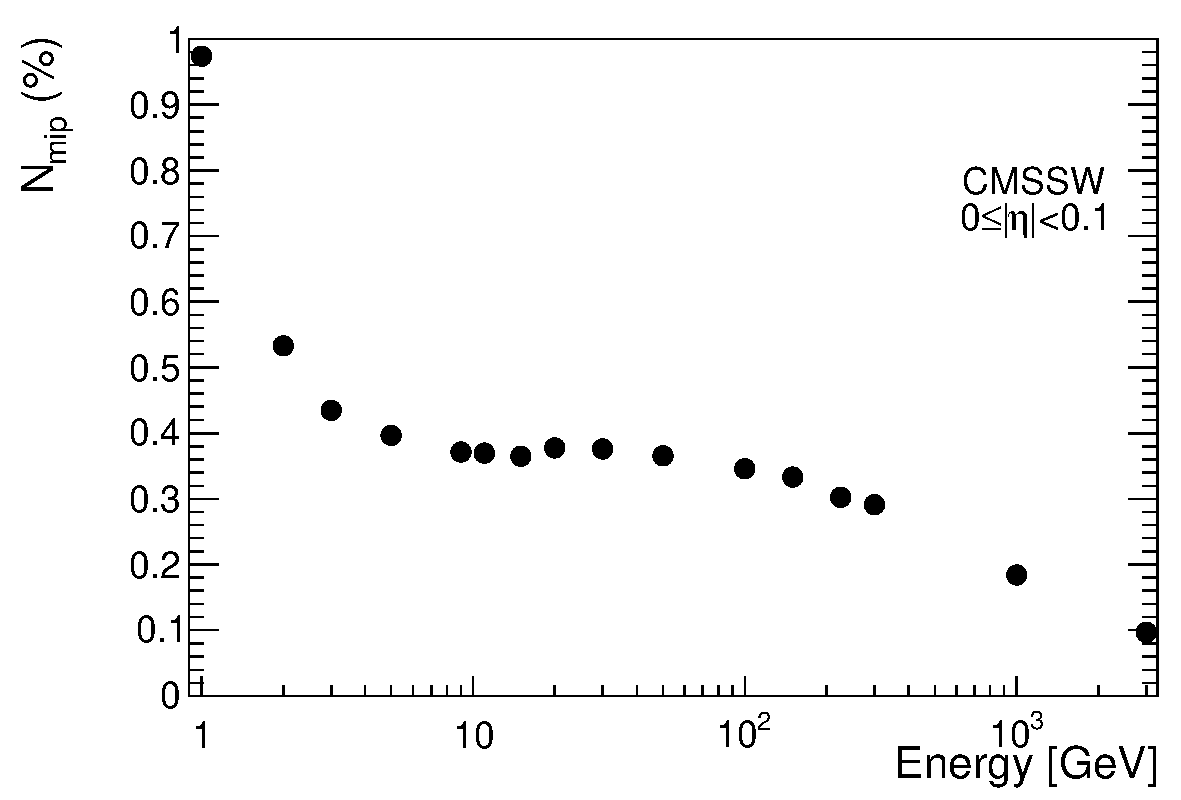
\includegraphics[width=0.49\textwidth]{figures/fs_plot_mip_ieta1.pdf}
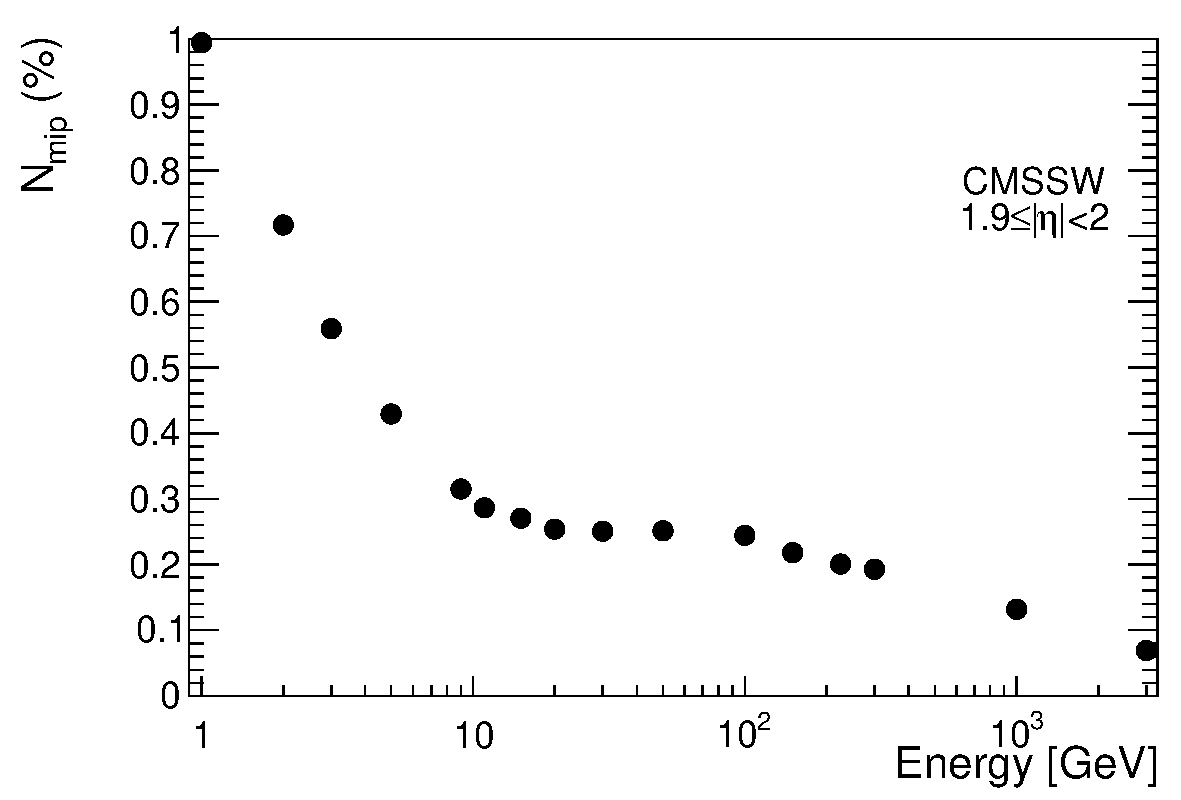
\includegraphics[width=0.49\textwidth]{figures/fs_plot_mip_ieta20.pdf}
\caption{Plots of MIP percentage vs. energy for $i\eta = 1$ (in the barrel) and $i\eta = 20$ (in the endcap).}
\label{fig:mippct}
\end{center}
\end{figure}

\begin{figure}[hbtp]
\begin{center}
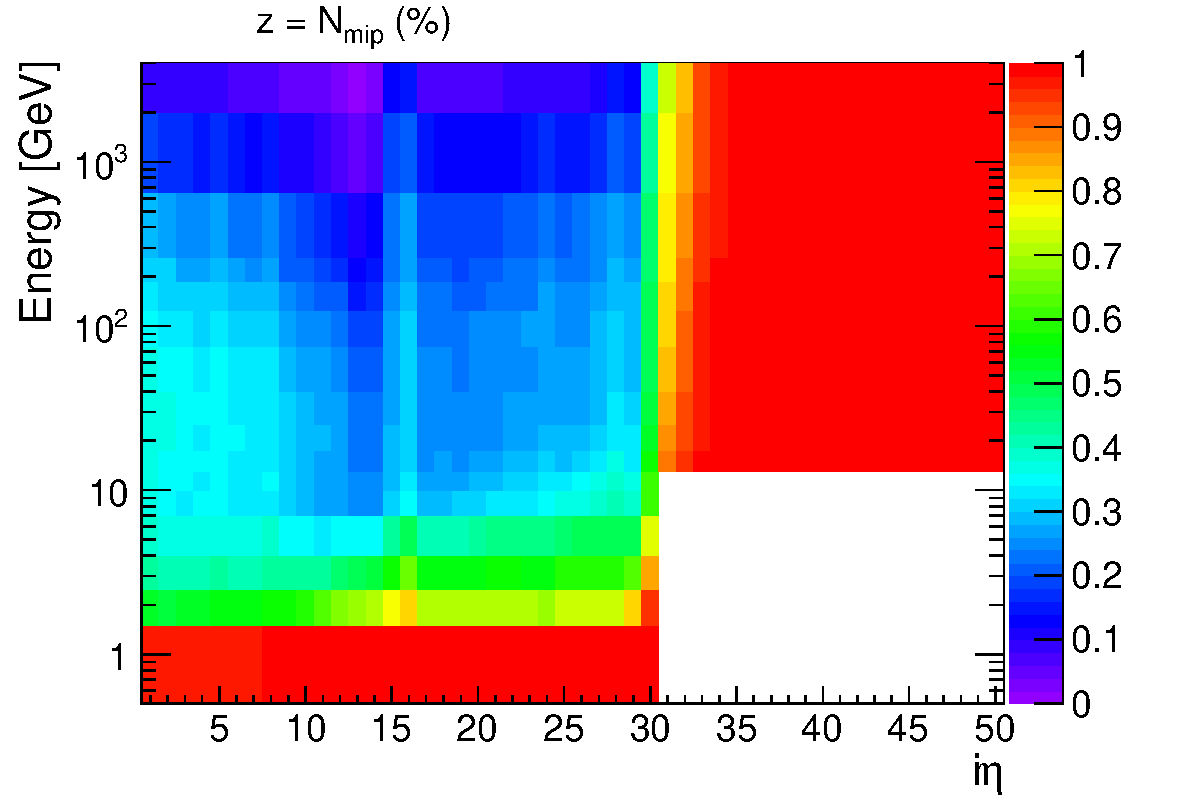
\includegraphics[width=0.95\textwidth]{figures/all_mip.pdf}
\caption{Plots of MIP percentage vs. energy and $\eta$ for the entire calorimeter system.}
\label{fig:allmippct}
\end{center}
\end{figure}

\section{Dose Rate Effects}

\subsection{Dose Rate Effect Models}

\subsection{Scintillator Radiation Damage Studies}